\chapter{Análise Estatística Não Paramétrica}
\label{chap:analise_estatistica_np}

Considerando que as distribuições das métricas de conectividade (diferença entre Pós e Pré) não se comportam de maneira normal (ver Capítulo~\ref{chap:analise_distribuicao_normalidade}), optamos por empregar testes estatísticos não paramétricos para comparar as condições de estimulação (\texorpdfstring{\textit{cathodic} versus \textit{sham}}{cathodic versus sham}). Essa escolha evita pressupostos inadequados sobre a distribuição dos dados e confere maior robustez às inferências.

Nesta etapa, foram aplicados os seguintes testes:
\begin{itemize}
    \item \textbf{Mann-Whitney U:} Teste para amostras independentes, comparando as condições para cada faixa de frequência e grupo de canais. O tamanho do efeito foi estimado pela fórmula:
    \[
    \text{effect size} = \frac{2\cdot \text{stat}}{n_{\text{cathodic}} \cdot n_{\text{sham}}} - 1.
    \]
    \item \textbf{Wilcoxon:} Teste para amostras pareadas, no qual os dados foram emparelhados por atleta, par de canais e faixa de frequência, permitindo uma comparação intraindividual entre as condições.
    \item \textbf{Kruskal-Wallis:} Teste para múltiplos grupos, empregado para comparar as condições quando os dados foram agrupados por faixa de frequência, com o tamanho do efeito estimado pela razão entre a estatística do teste e o número total de observações menos um.
\end{itemize}

Os testes foram realizados separadamente para cada uma das métricas de conectividade (\texttt{median\_plv\_diff}, \texttt{median\_pli\_diff} e \texttt{median\_cf\_plm\_diff}) e para os dois grupos de canais: \texttt{EEG\_EEG} e \texttt{EEG\_ECG}. Ressalta-se que, embora o código inclua procedimentos para remoção de dados nulos, na prática esses valores não estão presentes, servindo apenas para tratamento de exceções.

\section{Resultados dos Testes}

\subsection{\texorpdfstring{Métricas para \texttt{median\_pli\_diff}}{Métricas para median\_pli\_diff}}

\paragraph{Grupo EEG\_EEG:}
\begin{itemize}
    \item \textbf{Mann-Whitney U:} As faixas \emph{alpha}, \emph{delta}, \emph{gamma} e \emph{theta} apresentaram diferenças significativas (p-valores $< 0.001$), enquanto a faixa \emph{beta} teve um resultado marginal ($p \approx 0.051$).
    \item \textbf{Wilcoxon:} Os testes pareados indicaram significância robusta em todas as faixas, com tamanho de efeito em torno de $0.477$.
    \item \textbf{Kruskal-Wallis:} As faixas \emph{alpha}, \emph{delta}, \emph{gamma} e \emph{theta} apresentaram diferenças estatisticamente significativas, com a faixa \emph{beta} sendo marginalmente não significativa.
\end{itemize}

\subsection{\texorpdfstring{Métricas para \texttt{median\_cf\_plm\_diff}}{Métricas para median\_cf\_plm\_diff}}

\paragraph{Grupo EEG\_ECG:}
\begin{itemize}
    \item \textbf{Mann-Whitney U:} As faixas \emph{alpha}, \emph{beta} e \emph{delta} foram significativamente diferentes (p-valores $< 0.05$), enquanto as faixas \emph{gamma} e \emph{theta} não apresentaram significância.
    \item \textbf{Wilcoxon:} Todos os testes resultaram em p-valores extremamente baixos, com tamanhos de efeito de aproximadamente $0.358$.
    \item \textbf{Kruskal-Wallis:} As faixas \emph{alpha}, \emph{beta} e \emph{gamma} apresentaram diferenças significativas, enquanto as faixas \emph{delta} e \emph{theta} não demonstraram diferenças estatísticas.
\end{itemize}

\section{Discussão e Justificativa dos Métodos}

Os testes de normalidade indicaram violações significativas dos pressupostos de normalidade para as métricas de conectividade analisadas, o que justificou o uso de testes não paramétricos para comparar as condições de estimulação (\texttt{cathodic} versus \texttt{sham}). Esses métodos não dependem de pressupostos sobre a distribuição dos dados, oferecendo uma análise mais robusta e confiável, especialmente em cenários com alta variabilidade e a presença de outliers.

A aplicação conjunta de múltiplos testes (Mann-Whitney U, Wilcoxon e Kruskal-Wallis) permitiu uma avaliação abrangente das diferenças entre as condições, considerando tanto comparações entre grupos independentes quanto análises pareadas intraindividuais. Os resultados indicam que, para a maioria das faixas de frequência e para as métricas \texttt{median\_pli\_diff} e \texttt{median\_cf\_plm\_diff}, existem diferenças estatisticamente significativas entre as condições, reforçando a importância da modulação induzida pela estimulação.

Por outro lado, os achados para a \texttt{median\_pli\_diff} apresentaram maior variação, dependendo do teste estatístico e da faixa de frequência considerada, o que sugere uma sensibilidade maior dessa métrica a variações no processamento neural. Em suma, a escolha dos testes não paramétricos foi justificada pela não conformidade dos dados com a normalidade, e os resultados obtidos fornecem evidências sólidas de diferenças na sincronização de fase entre as condições experimentais, corroborando os efeitos da estimulação no contexto das análises de conectividade.

\section{Detecção de Outliers, Análise Bootstrap e Correções para Comparações Múltiplas}

Para aprimorar a qualidade dos dados e reduzir o impacto de pontos atípicos nas análises subsequentes, adotamos uma etapa de detecção e remoção de outliers utilizando o método ECOD (Empirical Cumulative Distribution-based Outlier Detection). O ECOD é especialmente adequado para nosso conjunto de dados devido à sua natureza não paramétrica, que permite identificar anomalias sem pressupor uma distribuição específica dos dados. Esse método estima a função de distribuição cumulativa empírica em cada dimensão e identifica como outliers os pontos que se desviam significativamente do comportamento esperado. Estudos demonstram que o ECOD supera diversas técnicas convencionais de detecção de outliers em termos de acurácia e eficiência \cite{li2022ecod}.

Aplicamos o ECOD considerando as métricas \texttt{median\_pli\_diff} e \texttt{median\_cf\_plm\_diff}. Inicialmente, o dataset continha 122915 entradas; após a aplicação do ECOD, aproximadamente 5,00\% dos dados foram identificados como outliers e removidos, aumentando a robustez das análises subsequentes.

Posteriormente, implementamos um robusto pipeline de análise baseado em bootstrap acelerado por GPU para o cálculo de intervalos de confiança BCa (Bias-Corrected and Accelerated). Esse método é particularmente robusto, pois ajusta tanto o viés quanto a aceleração da distribuição bootstrap, permitindo capturar assimetrias e a influência residual de outliers nos dados. Embora computacionalmente custoso, o método BCa é amplamente reconhecido como uma das abordagens mais precisas para a estimação de intervalos de confiança em situações onde os pressupostos de normalidade não são atendidos. Optamos por esse método em detrimento de outras técnicas devido à sua capacidade de corrigir distorções na distribuição da estatística estimada.

Para avaliar a significância estatística após as múltiplas comparações, utilizamos a função \texttt{multipletests} da biblioteca Python \texttt{statsmodels} com o método Bonferroni. Este procedimento gera uma nova coluna, denominada \texttt{bonferroni\_corrected\_p}, onde o p-valor original (bruto) é multiplicado pelo número total de testes (neste caso, 11.346). Dessa forma, declara-se um efeito significativo quando \(\texttt{bonferroni\_corrected\_p} < 0.05\).

Além disso, nosso pipeline incluiu o cálculo de tamanhos de efeito utilizando diversas métricas, tais como:
\begin{itemize}
    \item \textbf{Cohen's d} e \textbf{Hedges' g}: que quantificam a magnitude da diferença entre as condições em termos de desvios-padrão;
    \item \textbf{Rank-Biserial Correlation (RBC)}: derivado do teste de Wilcoxon, que fornece uma interpretação robusta baseada em postos.
\end{itemize}
Essas métricas complementares permitem uma avaliação abrangente do efeito da estimulação e possibilitam a comparação dos resultados com os intervalos de confiança BCa e os p-valores corrigidos pelo método Bonferroni. Na tabela de resultados em anexo, os leitores encontrarão também as correções de Holm e FDR-BH, bem como os tamanhos de efeito calculados, permitindo uma comparação completa entre os diferentes métodos.

Em resumo, nossa abordagem compreende as seguintes etapas:
\begin{enumerate}
    \item \textbf{Detecção de Outliers:} Utilizamos o método ECOD para identificar e remover aproximadamente 5\% dos dados considerados anômalos, garantindo a robustez das análises.
    \item \textbf{Análise Bootstrap com GPU:} Implementamos o cálculo de intervalos de confiança BCa, estimando viés, erro padrão e tamanhos de efeito por meio de reamostragem acelerada, assegurando precisão mesmo em distribuições assimétricas.
    \item \textbf{Testes Não Paramétricos e Correção para Comparações Múltiplas:} Aplicamos testes não paramétricos, como o teste de Wilcoxon para dados emparelhados, e corrigimos os p-valores utilizando o método Bonferroni (além de outras correções complementares), minimizando o risco de erros do tipo I.
\end{enumerate}

Os resultados deste processamento serão apresentados em detalhes nos anexos, permitindo a comparação dos resultados obtidos com e sem a remoção de outliers, bem como a análise dos diferentes tamanhos de efeito e métodos de correção.

\section{Distribuição de Tamanhos de Efeito e p-valores}
\label{sec:effect_size_distribution}

Nesta etapa, examinamos a distribuição das estimativas de tamanho de efeito (\emph{Cohen's d}, \emph{Hedges' g} e \emph{Wilcoxon RBC}) e dos valores-p (brutos e corrigidos por Bonferroni) para as análises de PLI (EEG-EEG) e CF-PLM (EEG-ECG), considerando cenários com e sem outliers. A Figura~\ref{fig:effectsizehist_all} ilustra, em quatro subfiguras, como essas métricas se distribuem ao longo dos pares de canal e faixas de frequência analisados.

\begin{figure}[htb]
    \centering
    % Subfigura 1: PLI (EEG-EEG), Sem Outliers
    \subfloat[Sem Outliers -- PLI (EEG-EEG)]{
        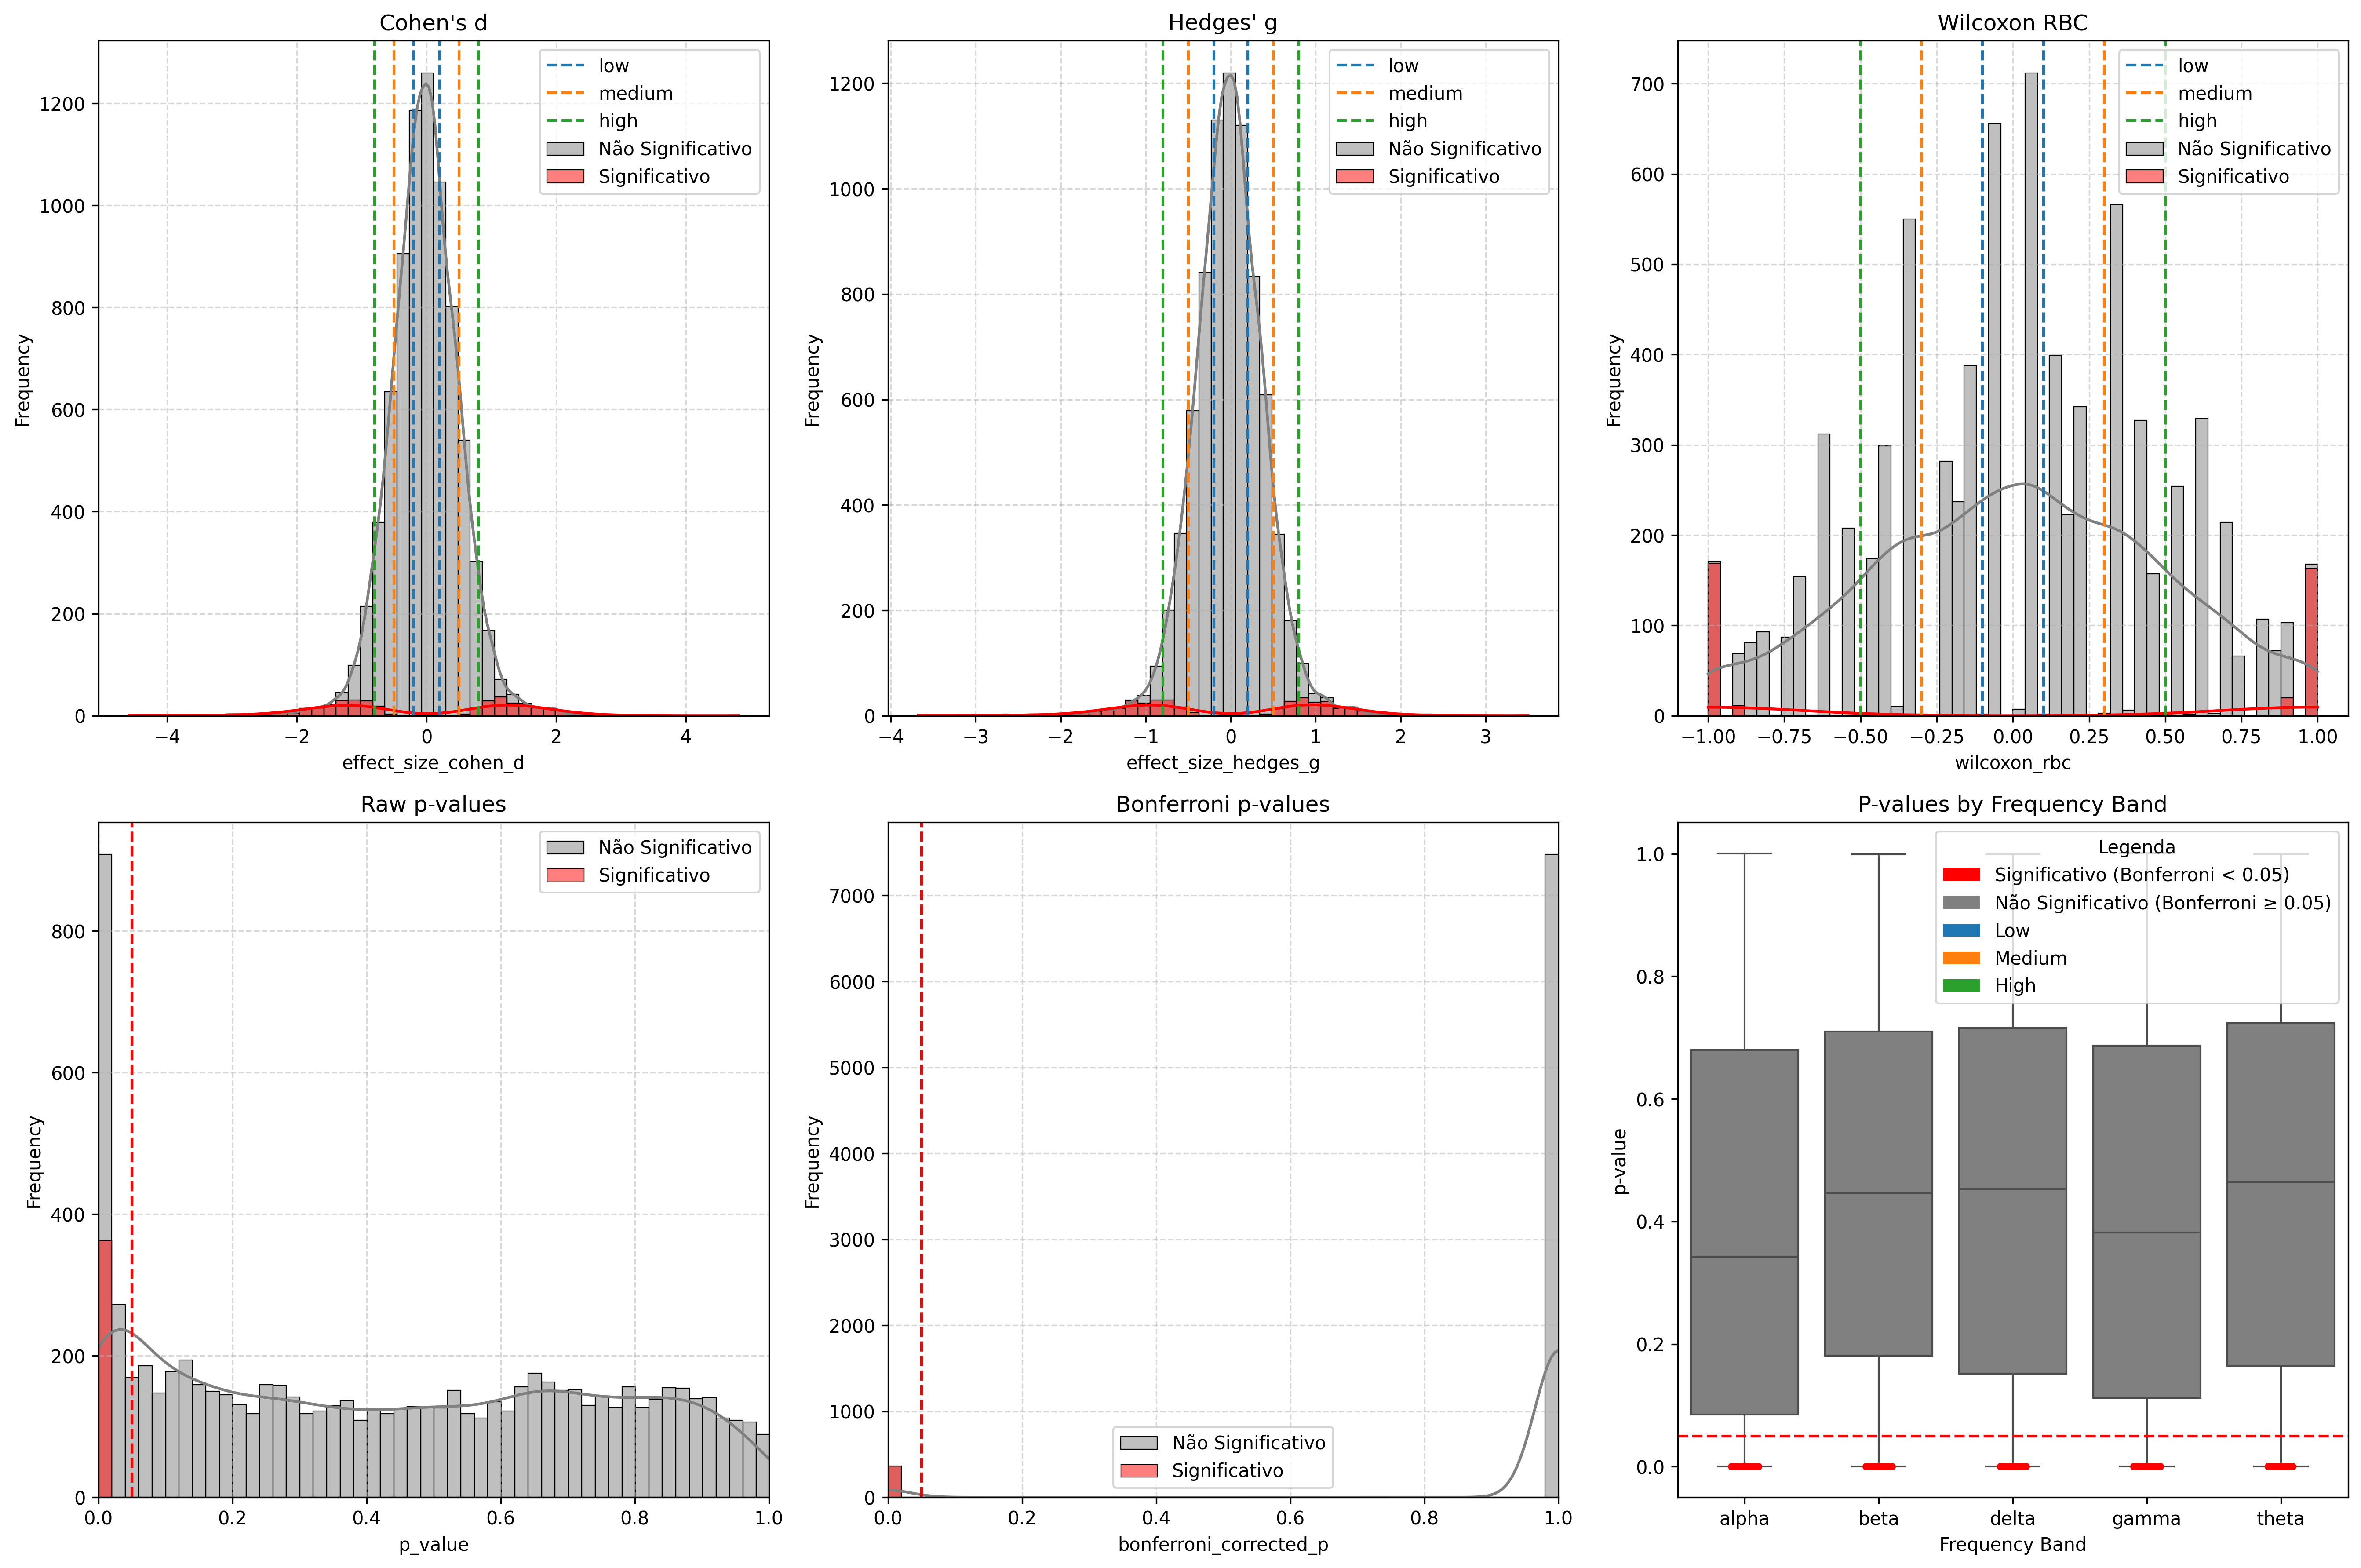
\includegraphics[width=0.45\textwidth]{figs/7_bootstrap_results_analysis/1_effect_size_histograms/Effect_Size_Histograms_PLI_EEGEEG_Sem_Outliers.png}
    }
    \quad
    % Subfigura 2: CF-PLM (EEG-ECG), Sem Outliers
    \subfloat[Sem Outliers -- CF-PLM (EEG-ECG)]{
        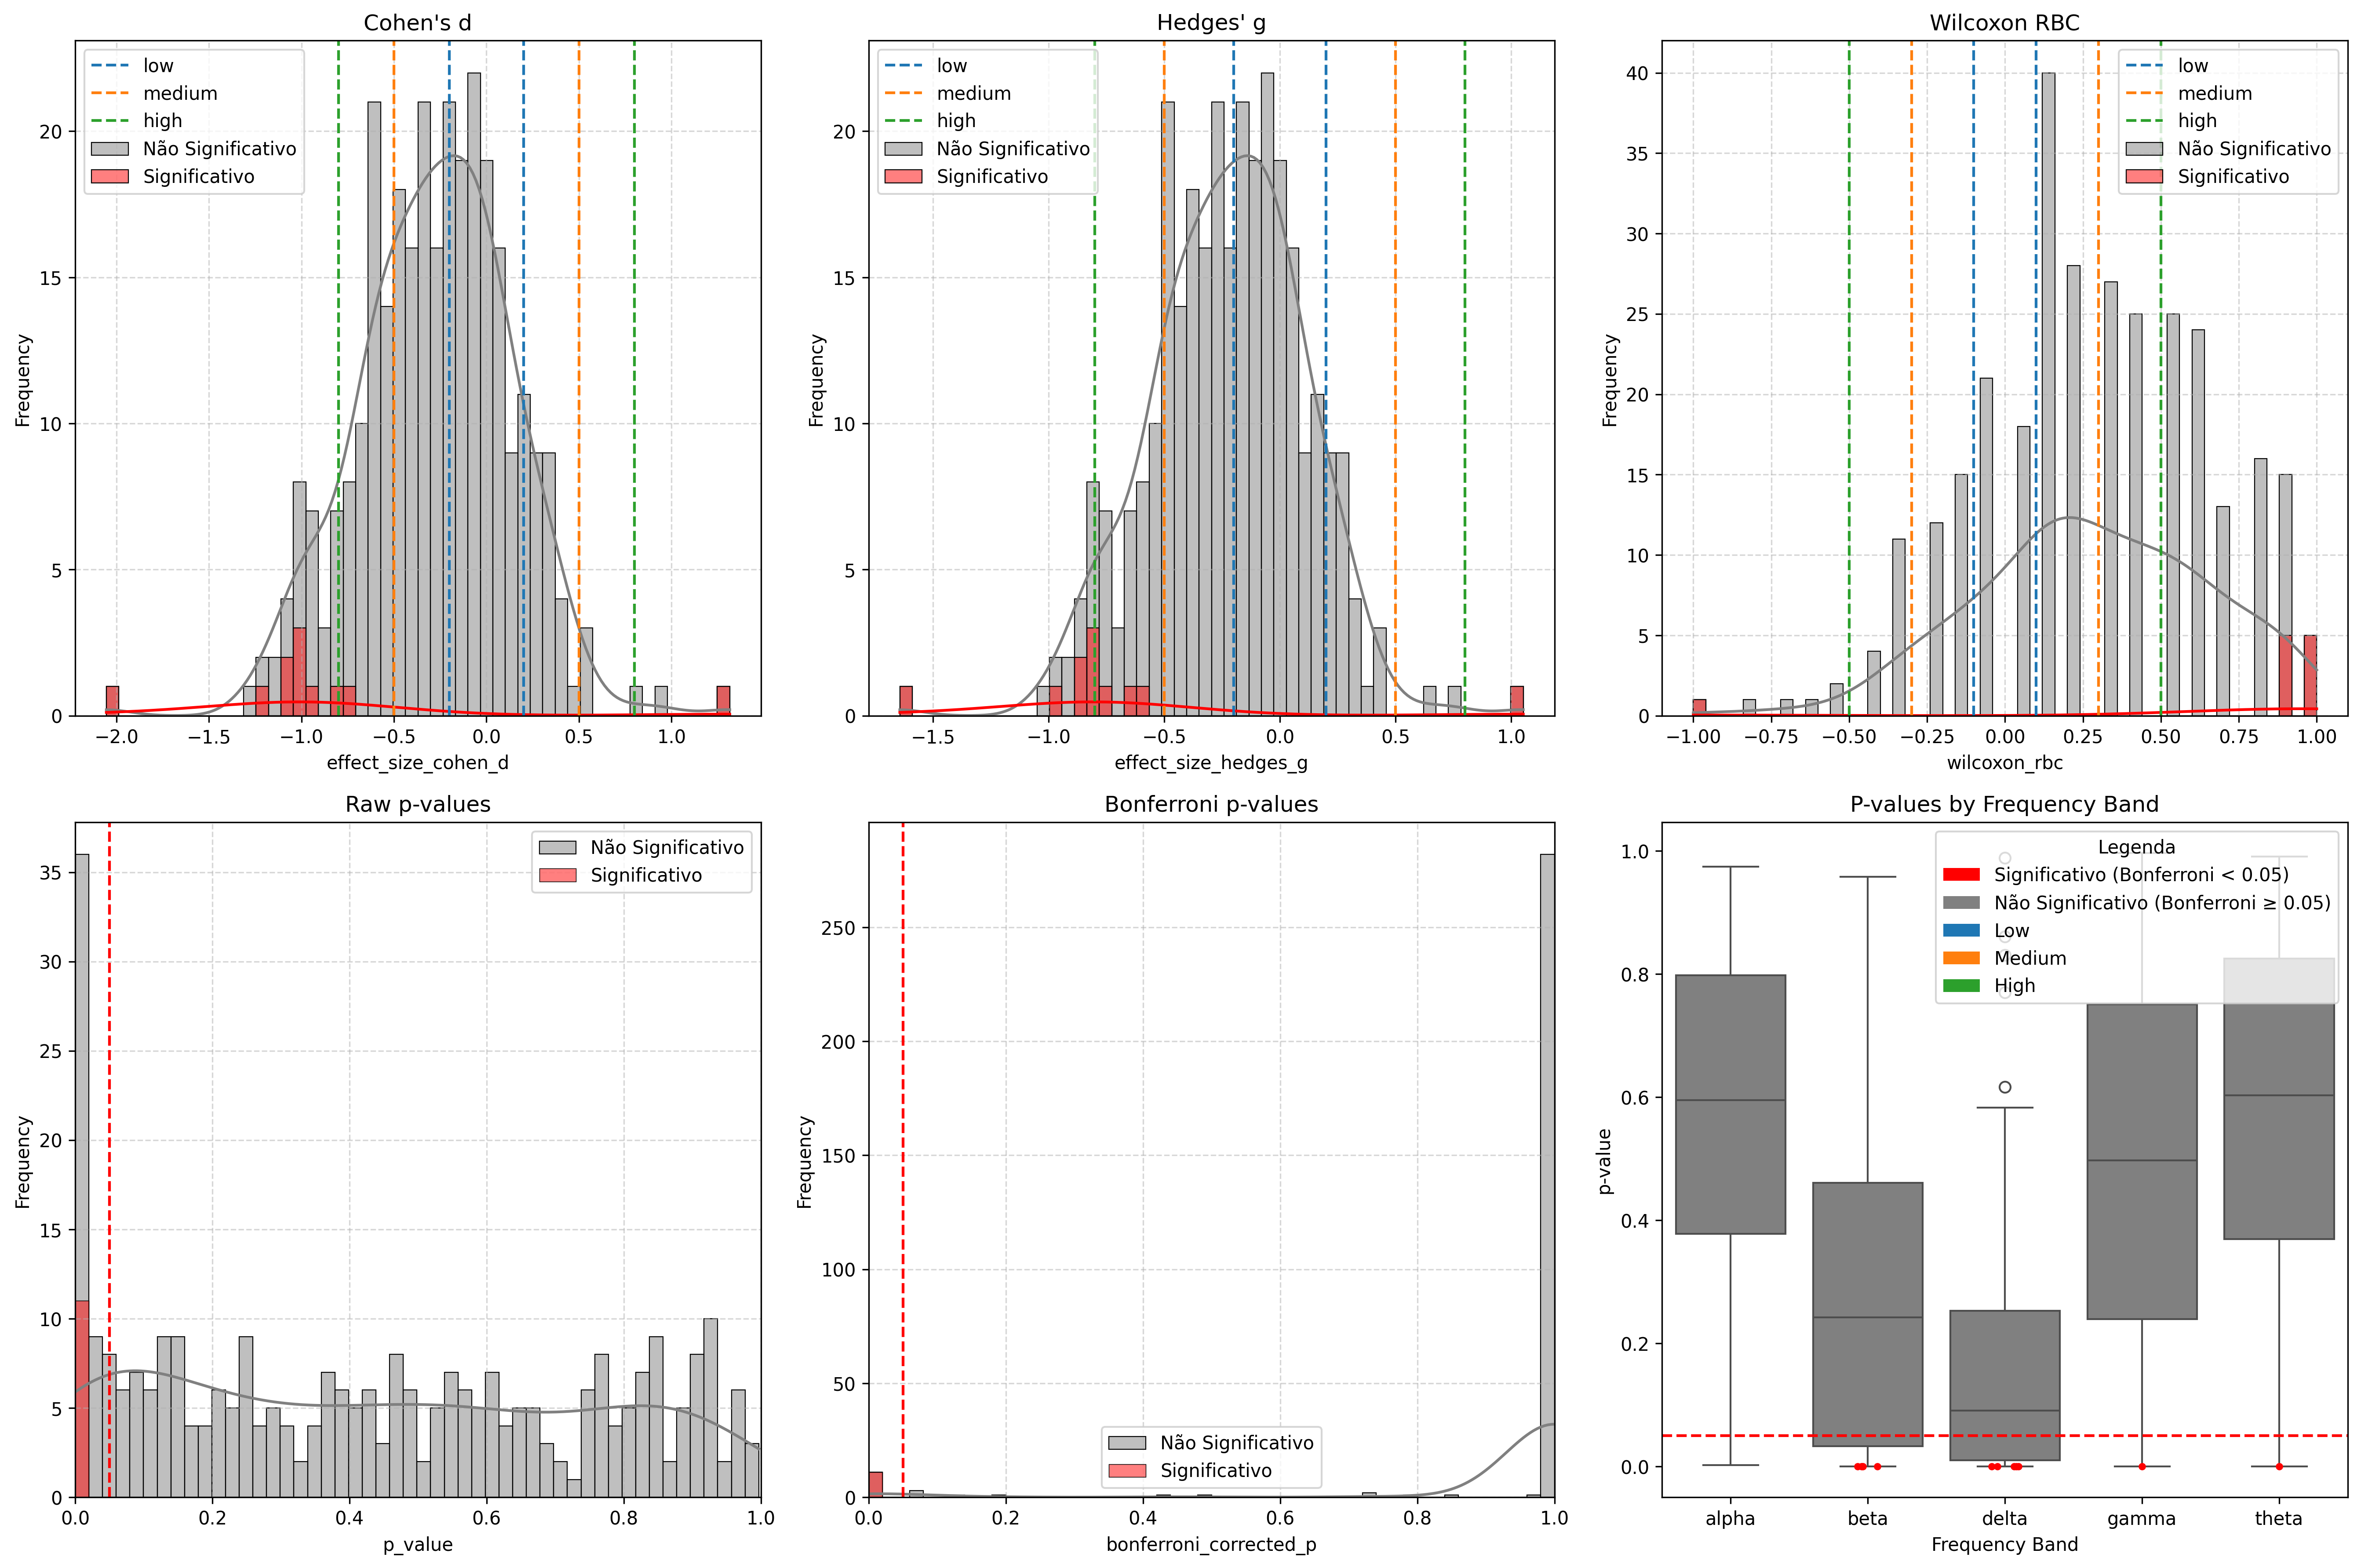
\includegraphics[width=0.45\textwidth]{figs/7_bootstrap_results_analysis/1_effect_size_histograms/Effect_Size_Histograms_CFPLM_EEGECG_Sem_Outliers.png}
    }
    \\
    % Subfigura 3: PLI (EEG-EEG), Com Outliers
    \subfloat[Com Outliers -- PLI (EEG-EEG)]{
        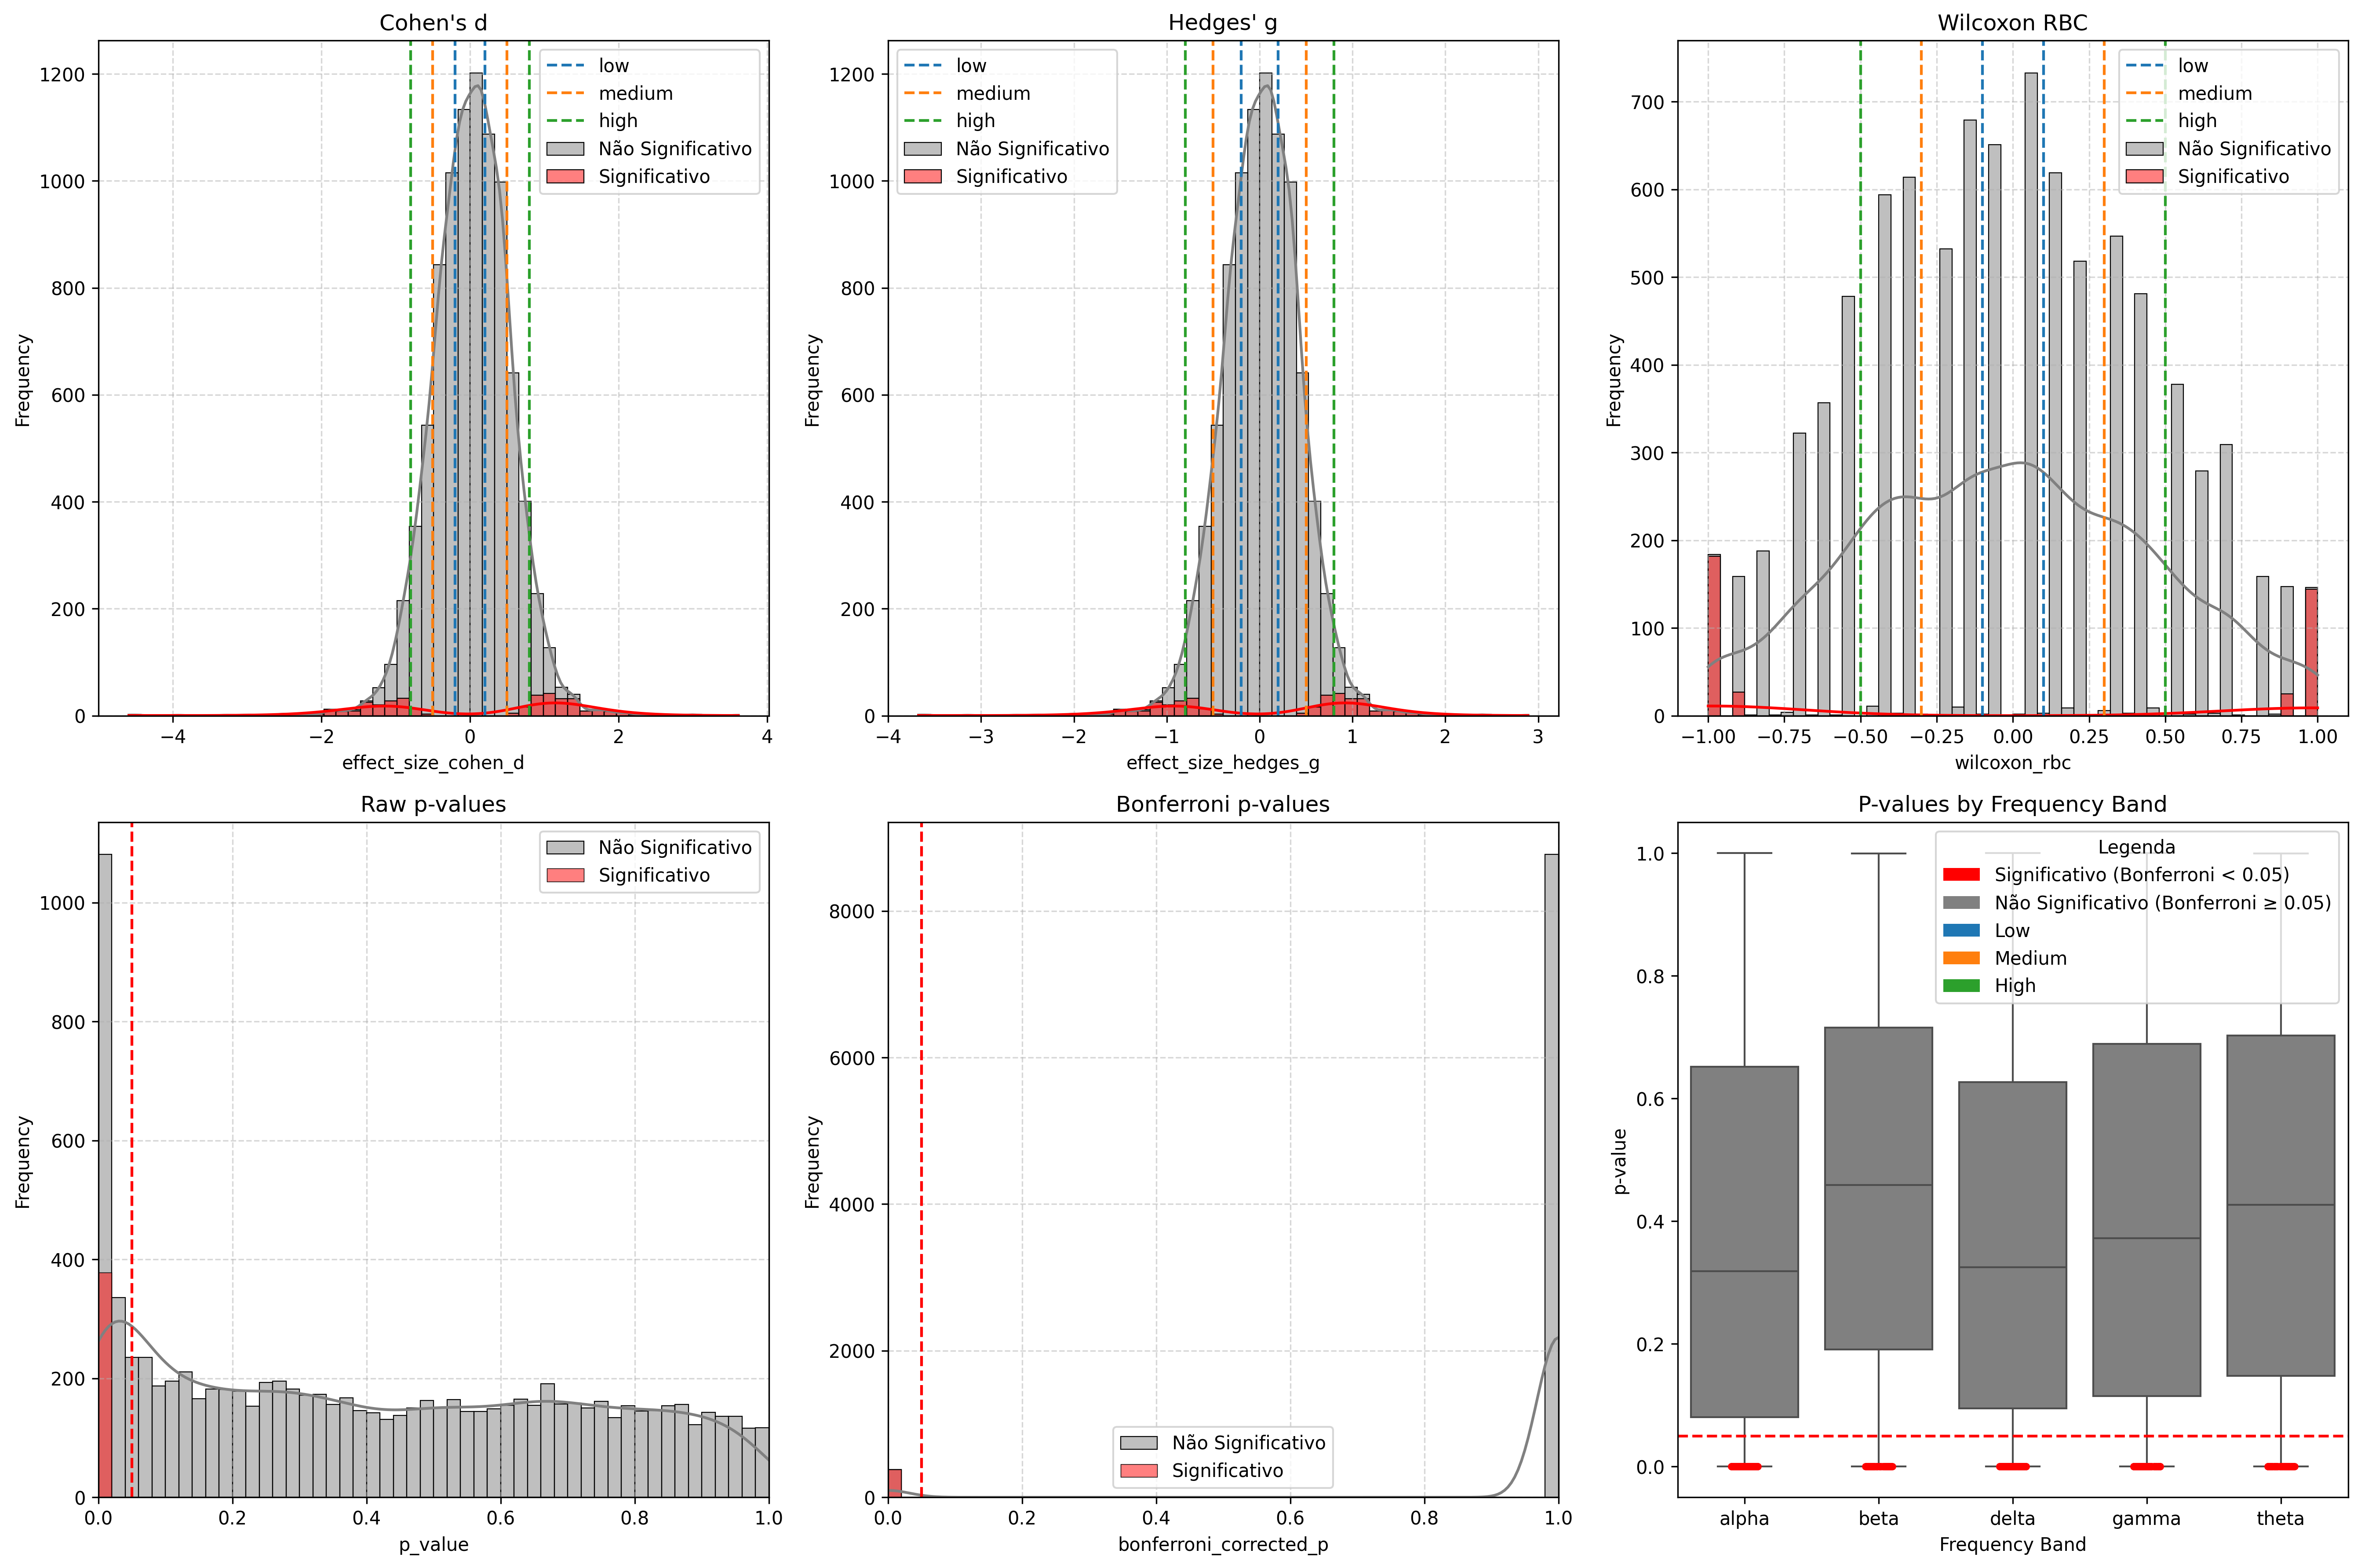
\includegraphics[width=0.45\textwidth]{figs/7_bootstrap_results_analysis/1_effect_size_histograms/Effect_Size_Histograms_PLI_EEGEEG_Com_Outliers.png}
    }
    \quad
    % Subfigura 4: CF-PLM (EEG-ECG), Com Outliers
    \subfloat[Com Outliers -- CF-PLM (EEG-ECG)]{
        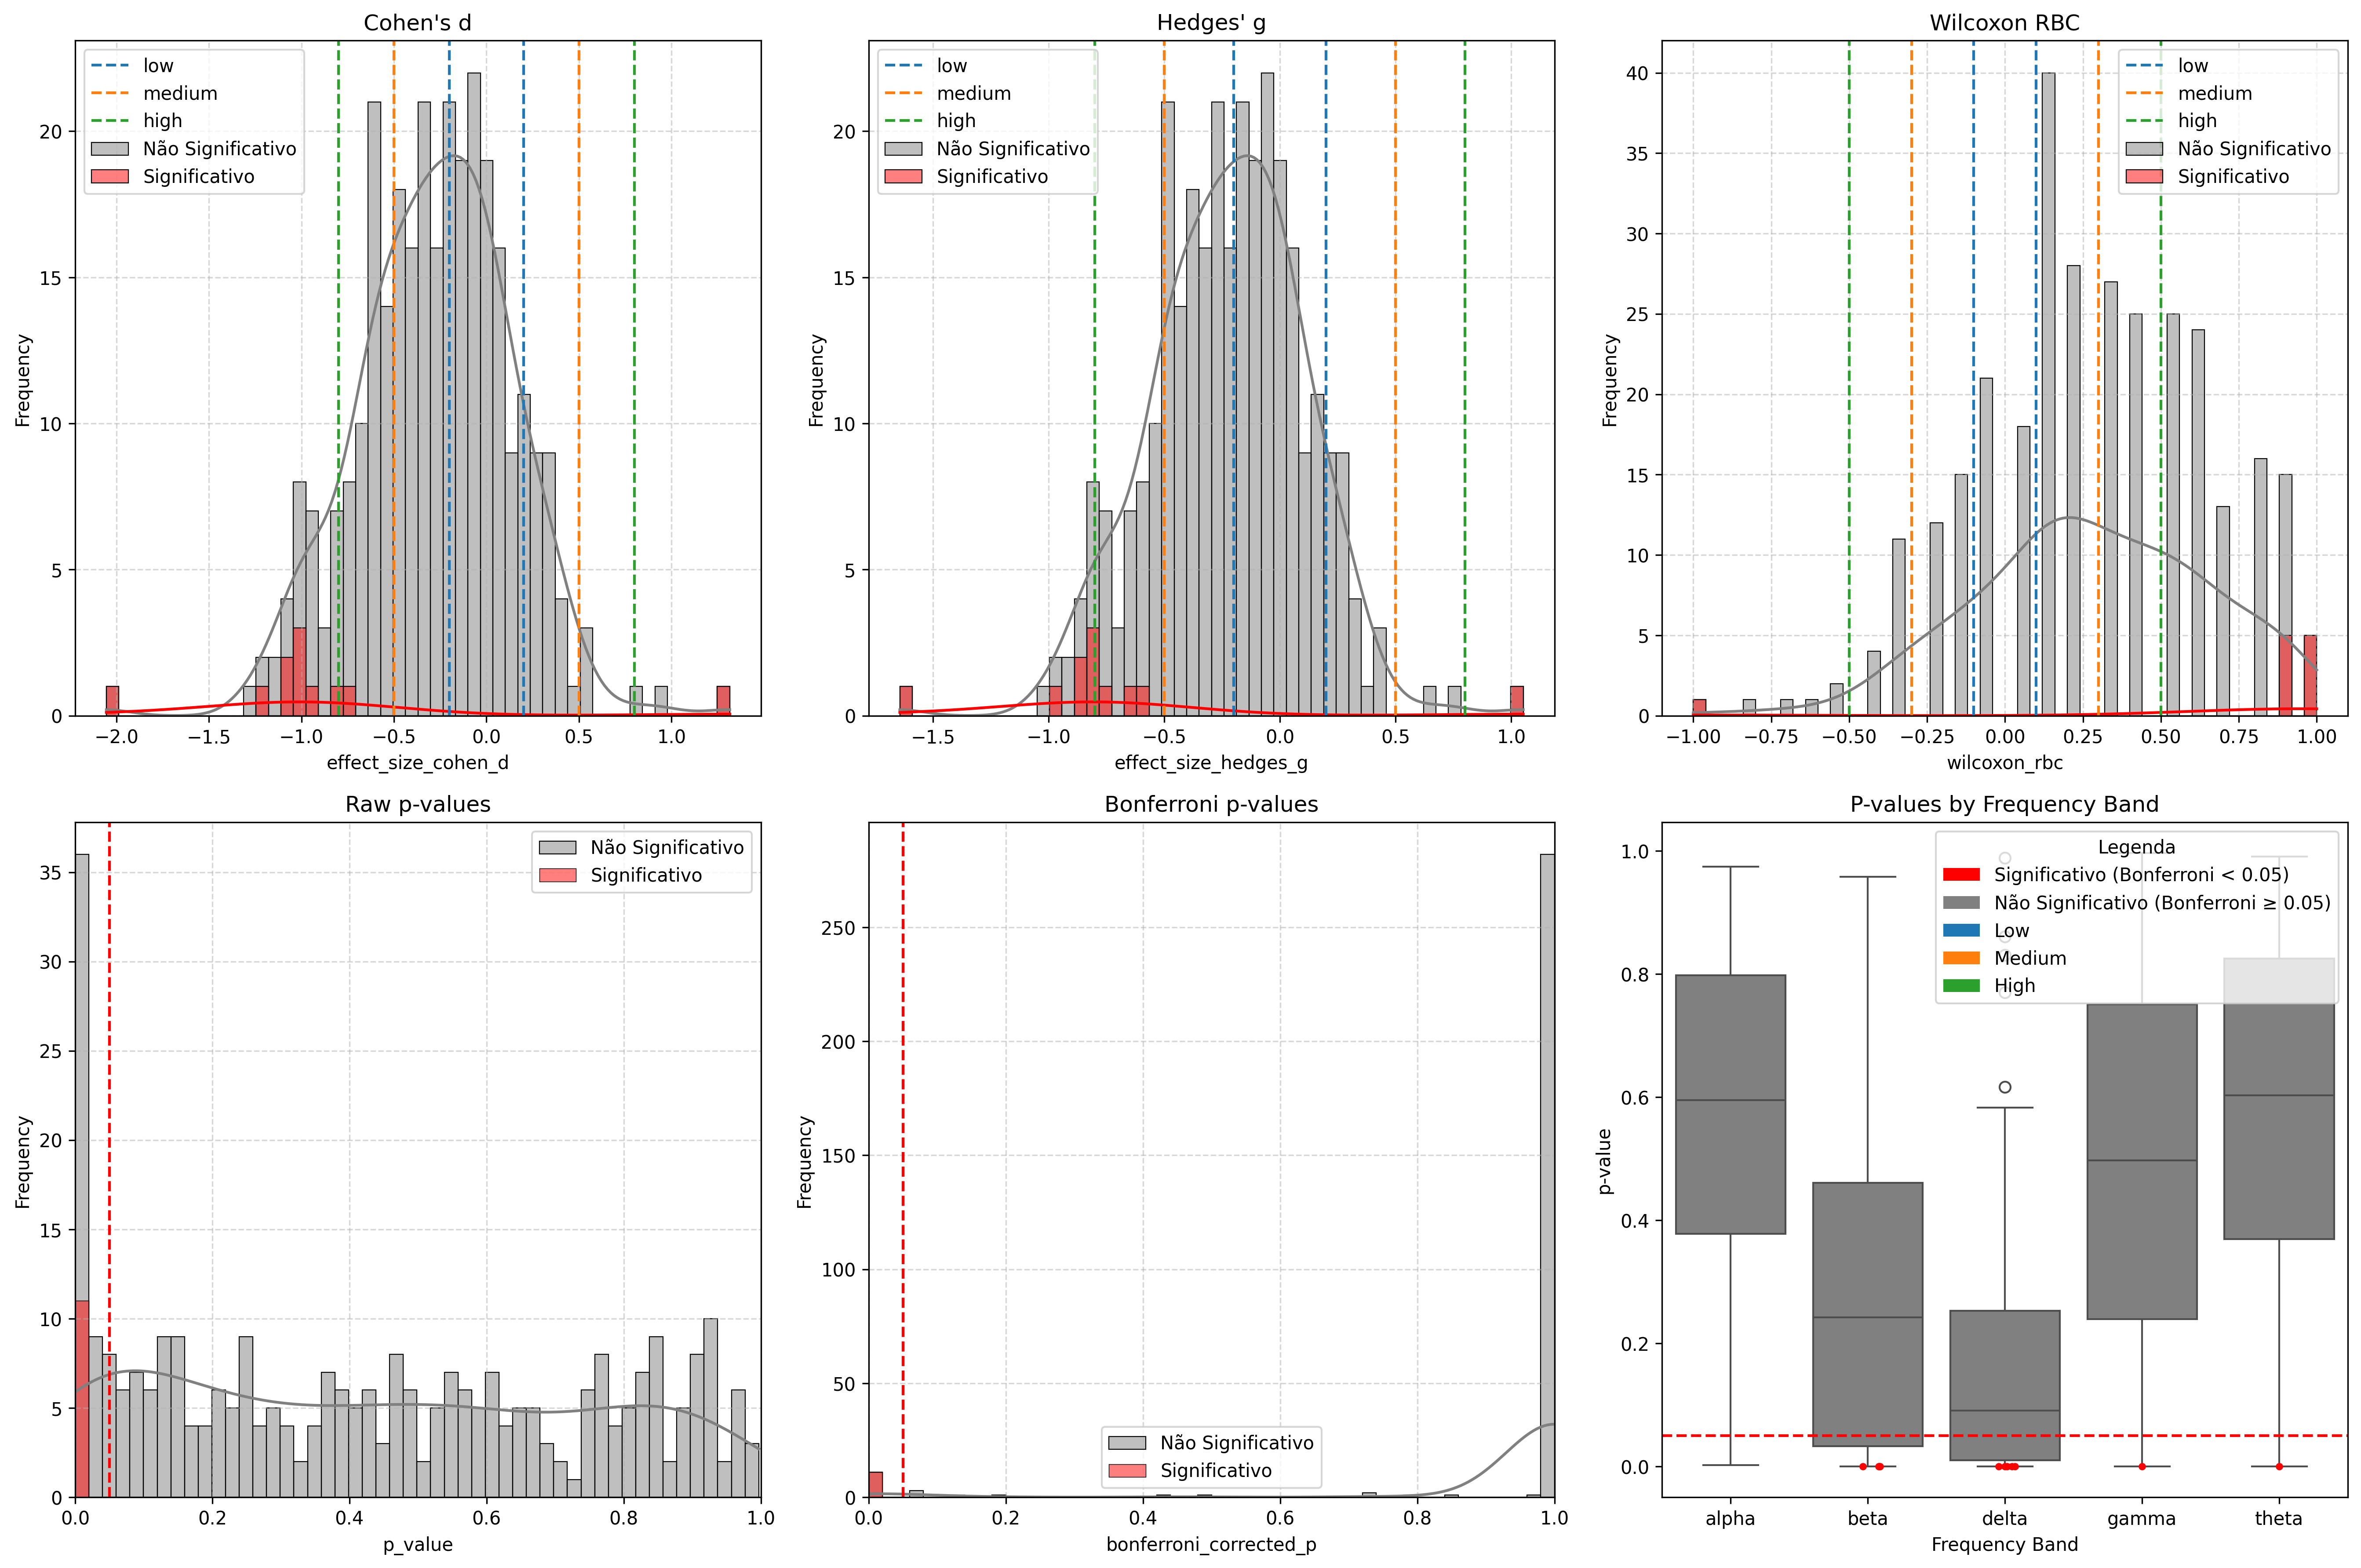
\includegraphics[width=0.45\textwidth]{figs/7_bootstrap_results_analysis/1_effect_size_histograms/Effect_Size_Histograms_CFPLM_EEGECG_Com_Outliers.png}
    }
    \caption[Distribuições de tamanhos de efeito e valores-p]{Distribuição das métricas de tamanho de efeito (\emph{Cohen's d}, \emph{Hedges' g} e \emph{Wilcoxon RBC}) e dos valores-p (brutos e corrigidos por Bonferroni) para PLI (EEG-EEG) e CF-PLM (EEG-ECG), em cenários com e sem outliers. O \emph{Wilcoxon RBC} e o p-valor corrigido por Bonferroni (vertical tracejada vermelha em $p=0.05$) são enfatizados como as métricas mais robustas para, respectivamente, o tamanho de efeito e a significância estatística.}
    \label{fig:effectsizehist_all}
\end{figure}
\subsection{Distribuição dos Tamanhos de Efeito}

\paragraph{Cohen's d e Hedges' g}
\begin{itemize}
    \item A maior parte dos valores concentra-se em torno de zero, indicando que, para a maioria dos pares, as diferenças entre as condições \emph{cathodic} e \emph{sham} são pequenas ou não significativas.
    \item Valores significativos (representados pelas barras vermelhas nos histogramas) tendem a se afastar de zero, sinalizando diferenças mais acentuadas. Por exemplo, valores de \emph{Cohen's d} ou \emph{Hedges' g} superiores a 0.5 (ou inferiores a -0.5) sugerem um efeito moderado, enquanto valores acima de 0.8 (ou inferiores a -0.8) indicam um efeito alto.
    \item Embora \emph{Hedges' g} difira de \emph{Cohen's d} ao aplicar uma correção para tamanhos amostrais pequenos, ambas as métricas exibem comportamentos semelhantes nos histogramas.
\end{itemize}

\paragraph{Wilcoxon RBC (Rank-Biserial Correlation)}
\begin{itemize}
    \item O \emph{Wilcoxon RBC} é derivado do teste não paramétrico de Wilcoxon e reflete a correlação de postos entre as condições, tipicamente variando de -1 a +1.
    \item Por não exigir pressupostos de normalidade, o RBC se mostra mais robusto no tratamento de dados heterogêneos e na presença de outliers.
    \item Valores acima de 0.3 ou abaixo de -0.3 sugerem um efeito moderado; valores acima de 0.5 (ou abaixo de -0.5) indicam um efeito alto, e quando se aproximam de ±1, as condições diferem de forma quase absoluta.
    \item Devido a essa robustez, o RBC foi escolhido como nosso principal indicador de tamanho de efeito nas análises subsequentes.
\end{itemize}

\subsection{Distribuição de p-valores (Brutos e Corrigidos)}

\begin{itemize}
    \item Os histogramas de p-valores brutos mostram uma forte concentração em torno de 1 (indicando resultados não significativos) e uma cauda próxima de 0 (sinalizando potenciais resultados significativos).
    \item Após a correção de Bonferroni (indicada pela linha vertical tracejada em \(p=0.05\)), muitos dos valores que eram marginalmente significativos foram deslocados para a região de não significância, evidenciando o caráter conservador deste método de correção.
    \item Devido ao elevado número de comparações, a utilização do método Bonferroni minimiza a probabilidade de falsos positivos, sendo adotado como critério principal para a significância estatística.
\end{itemize}


\subsection{Comparação Entre Cenários (Com e Sem Outliers)}
\begin{itemize}
    \item \textbf{Diferenças Mínimas:} De modo geral, a remoção de outliers reduz ligeiramente o número de casos significativos em EEG-EEG, mas não altera substancialmente a distribuição dos tamanhos de efeito ou dos p-valores. No caso do EEG-ECG, a diferença entre manter ou remover outliers é praticamente irrelevante.
    \item \textbf{PLI (EEG-EEG):} Com um número significativamente maior de pares (cada um dos 61 canais de EEG formando pares entre si), foram identificados entre 363 (com remoção de outliers) e 378 casos (sem remoção de outliers) significativos.
    \item \textbf{CF-PLM (EEG-ECG):} Em contraste, apenas 11 casos significativos foram observados, pois cada canal de EEG forma par com o único canal de ECG, resultando em um total menor de pares possíveis.
    \item \textbf{Robustez do RBC e do Bonferroni:} Independentemente da remoção de outliers, as comparações que apresentam valores elevados de \emph{Wilcoxon RBC} e p-valores corrigidos abaixo de 0.05 permanecem confiáveis, reforçando o valor dessas métricas na interpretação dos resultados.
\end{itemize}

Em síntese, os histogramas de \emph{Wilcoxon RBC} (indicador de tamanho de efeito) e os p-valores corrigidos por Bonferroni (indicador de significância estatística) demonstram claramente quais pares de canais se destacam por apresentar diferenças robustas entre as condições \emph{cathodic} e \emph{sham}. Embora \emph{Cohen's d} e \emph{Hedges' g} também sejam úteis para quantificar a magnitude do efeito, nossa análise enfatiza o RBC, devido à sua robustez, natureza não paramétrica e resiliência à heterogeneidade dos dados. Esses resultados embasam as análises topográficas e de rede apresentadas nas seções seguintes.

\subsection{Conclusões Principais}
\begin{itemize}
    \item A maior parte dos dados concentra-se em torno de zero para todas as métricas, refletindo pequenas diferenças entre as condições. Esse comportamento é consistente com o uso de métodos robustos de correção múltipla (por exemplo, Bonferroni) e o elevado número de comparações.
    \item Quando há significância estatística, os tamanhos de efeito se afastam notavelmente de zero (conforme evidenciado por \emph{Cohen's d}, \emph{Hedges' g} ou RBC), sugerindo diferenças substanciais e possivelmente relevantes do ponto de vista neurofisiológico.
    \item O \emph{Wilcoxon RBC} se mostra particularmente robusto para capturar tanto a direção quanto a magnitude das diferenças sem pressupor normalidade, motivo pelo qual será enfatizado nas próximas análises topográficas e na construção dos grafos de conectividade.
\end{itemize}

Assim, a análise dos histogramas de tamanhos de efeito e dos p-valores fornece um panorama inicial robusto: embora muitos pares não apresentem diferenças significativas, uma fração considerável exibe efeitos moderados ou altos, com p-valores corrigidos abaixo do limiar de significância. Esses achados embasam investigações posteriores, que buscarão caracterizar a localização e as faixas de frequência onde a neuromodulação exerce impacto mais pronunciado.


\section{Análise de Rede para PLI (EEG-EEG)}
\label{sec:rede_pli_eeg}

Nesta seção, analisamos as redes de conexões significativas obtidas pela métrica PLI para pares EEG-EEG, segmentadas por bandas de frequência, considerando os cenários com e sem outliers. Cada nó representa um canal EEG, e o número adjacente indica o total de conexões significativas envolvendo esse canal. Linhas vermelhas representam conexões com valores de \emph{Wilcoxon RBC} tendendo a +1, indicando conexões robustas.

Apresentamos aqui apenas exemplos representativos das redes (por exemplo, na banda Alpha), enquanto a análise completa, abrangendo todas as bandas e cenários, pode ser encontrada no \textbf{Apêndice \ref{apendice:pli_eeg_eeg}}.

\begin{figure}[htb]
  \centering
  \includegraphics[width=0.75\textwidth]{figs/7_bootstrap_results_analysis/2_network_graphs/PLI_EEG-EEG_Sem_Outliers/Banda_Alpha_(8_Hz_a_13_Hz)_-_Análise_de_Rede_-_PLI_EEG-EEG_Sem_Outliers.png}
  \caption{Exemplo da rede de conexões significativas na banda Alpha (8--13\,Hz) para PLI (EEG-EEG) no cenário sem outliers. Observa-se um núcleo central de canais altamente conectados, sugerindo forte sincronização.}
  \label{fig:exemplo_rede_pli_alpha_sem}
\end{figure}

\subsection{Resumo das Comparações (PLI EEG-EEG)}

A comparação detalhada entre os cenários com e sem outliers revela que:
\begin{itemize}
    \item \textbf{Topologia Similar:} A estrutura das redes permanece praticamente inalterada entre os cenários, indicando que a métrica PLI é robusta mesmo após a remoção de outliers.
    \item \textbf{Redução Ligeira:} A remoção de outliers resulta em uma leve redução no número de conexões significativas, mas não altera substancialmente a estrutura geral da rede.
    \item \textbf{Consistência dos Hubs:} Os canais com maior centralidade permanecem consistentes entre os cenários, reforçando a confiabilidade dos achados.
\end{itemize}

Para uma análise detalhada de todas as bandas e cenários, consulte o \textbf{Apêndice \ref{apendice:pli_eeg_eeg}}.

\section{Análise de Rede para CF-PLM (EEG-ECG, Cross-frequency)}
\label{sec:rede_cfplm_eeg_ecg}

Nesta seção, avaliamos as redes de conectividade \textbf{cross-frequency} entre EEG e ECG utilizando a métrica CF-PLM. Como os resultados mostraram padrões relativamente estáveis entre os cenários analisados, apresentamos aqui um \textbf{exemplo representativo} na banda Beta (13--30\,Hz). A análise completa para todas as bandas pode ser encontrada no \textbf{Apêndice \ref{apendice:cfplm_eeg_ecg}}.

\begin{figure}[htb]
  \centering
  \includegraphics[width=0.75\textwidth]{figs/7_bootstrap_results_analysis/2_network_graphs/CF-PLM_EEG-ECG_Sem_Outliers/Banda_Beta_(13_Hz_a_30_Hz)_-_Análise_de_Rede_-_CF-PLM_EEG-ECG_Sem_Outliers.png}
  \caption{Exemplo da rede CF-PLM na banda Beta (13--30\,Hz) para EEG-ECG sem outliers. Apesar da rede ser relativamente esparsa, os pares significativos indicam uma sincronização robusta.}
  \label{fig:exemplo_rede_cfplm_beta_sem}
\end{figure}

\subsection{Resumo das Comparações (CF-PLM EEG-ECG)}

As comparações entre os cenários com e sem outliers evidenciam que:
\begin{itemize}
    \item \textbf{Topologia Inalterada:} Tanto a estrutura quanto a quantidade de pares significativos permanecem praticamente inalteradas entre os dois cenários, indicando que os resultados são independentes da remoção de outliers.
    \item \textbf{Número Consistente de Pares:} O número total de pares significativos é idêntico (11 casos), sugerindo alta robustez dos efeitos cross-frequency detectados.
    \item \textbf{Consistência dos Achados:} Todos os pares significativos apresentam \emph{Wilcoxon RBC} igual a +1, reforçando a consistência dos achados.
\end{itemize}

Para mais detalhes e visualização completa das redes de conectividade, consulte o \textbf{Apêndice \ref{apendice:cfplm_eeg_ecg}}.

\subsection{Conclusões das Análises de Rede}
\begin{itemize}
    \item A análise de rede para PLI (EEG-EEG) evidencia que, mesmo com a remoção de outliers, a topologia das redes permanece robusta, com canais centrais consistentes, o que confirma a eficácia da métrica em capturar a sincronização entre os canais cerebrais.
    \item A análise de rede para CF-PLM (EEG-ECG) mostra que os efeitos cross-frequency são altamente robustos, com um número fixo de pares significativos e valores consistentes de \emph{Wilcoxon RBC}.
\end{itemize}

Esses achados fundamentam as análises topográficas e de rede que serão apresentadas nas seções seguintes.